\section{Evaluation}\label{sec:evaluation}

\begin{table}[!t]
\begin{small}
\begin{center}
\begin{tabular}{|l|r|r|r|r|r|}
\hline
\multirow{2}{*}{Referring Expressions} & \multicolumn{2}{|c|}{Corpus} & \multicolumn{2}{|c|}{Algorithm} & Accuracy \\ \cline{2-6} 
 & \#Cor & \multicolumn{1}{|c|}{\%Cor} & \multicolumn{1}{|c|}{\#Alg} & \multicolumn{1}{|c|}{\%Alg} & \multicolumn{1}{|c|}{\%Acc} \\
\hline
ball,green                                    & 91 & 65.00 & 6376 & 63.76 & 63.76 \\
ball,green,small                              & 23 & 16.43 & 3440 & 34.40 & 16.43 \\
ball,green,small,on-top(blue,cube,large)      &  8 &  5.71 &    0 &  0.00 &  0.00\\
ball,green,on-top(blue,cube)                  &  5 &  3.57 &    0 &  0.00 &  0.00\\
ball,green,on-top(blue,cube,large)            &  5 &  3.57 &    0 &  0.00 &  0.00\\
ball,green,small,on-top(blue,cube)            &  2 &  1.43 &    0 &  0.00 &  0.00\\
ball,on-top(cube)                             &  1 &  0.71 &   27 &  0.27 &  0.27 \\
ball,green,small,on-top(blue,cube,large,left) &  1 &  0.71 &    0 &  0.00 &  0.00\\
ball,small,on-top(cube,large)	              &  1 &  0.71 &    2 &  0.02 &  0.02 \\
ball,green,top                                &  1 &  0.71 &    0 &  0.00 &  0.00\\
ball,small,on-top(cube)                       &  1 &  0.71 &    3 &  0.03 &  0.03 \\
ball,green,on-top(cube)                       &  1 &  0.71 &    0 &  0.00 &  0.00\\
ball,front,green                              &  0 &  0.00 &   97 &  0.97 &  0.00\\
ball,front,green,small                        &  0 &  0.00 &   13 &  0.13 &  0.00\\
ball,front,top                                &  0 &  0.00 &   12 &  0.12 &  0.00\\
ball,green,left	                              &  0 &  0.00 &   11 &  0.11 &  0.00\\
ball,top                                      &  0 &  0.00 &   10 &  0.10 &  0.00\\
ball,green,left,small                         &  0 &  0.00 &    5 &  0.05 &  0.00\\
ball,left,top                                 &  0 &  0.00 &    2 &  0.02 &  0.00\\
ball,small,top                                &  0 &  0.00 &    1 &  0.01 &  0.00\\
ball,front,on-top(cube,left)                  &  0 &  0.00 &    1 &  0.01 &  0.00\\
\hline
Total & 140 & 100.00 & 10000 & 100 & 80.51 \\
\hline
\end{tabular}
\caption{REs in the corpus and those produced by our algorithm for Figure~\ref{GRE3D7-stimulus}\label{results-algo-fig3}}
\vspace*{-.5cm}
\end{center}
\end{small}
\end{table}

We present a quantitative evaluation of the algorithm proposed. 
In particular, we show that the probabilistic refinement algorithm with overspecification is able to generate a distribution of REs similar to that observed in corpora.
%, even when no corpus specific for a given target object is available. 
We discuss in detail the experiments we run for the scene shown in Figure~\ref{GRE3D7-stimulus} (Scene 3 in the GRE3D7 corpus), then summarize the results for the other seven scenes we used for testing. 


Using \puse\ learned as described in Section~\ref{sec:learning} and running 
our algorithm 10000 times, we obtain 14 different referring expressions 
for Figure~\ref{GRE3D7-stimulus}.  It is already interesting to see that with the 
\puse\ values learned from the corpus the algorithm generate only a small set of RE with a high probability. 
Of these 14 different REs, 5 are the most frequent REs found in the corpus of 140 REs associated to the Scene; indeed, 98\% of the utterances generated by the algorithm for this scene appear in the corpus.  
The remaining 9 REs generated by the algorithm, not present in the corpora, are very natural as can be observed in Table~\ref{results-algo-fig3}.
The table lists the REs in the corpus and the RE generated by the algorithm using the learned \puse. For each RE, we indicate the number of times it appears in the corpus (\#Cor), the proportion it represents (\%Cor), the number of times it is generated by our algorithm (\#Alg) and the proportion it represents (\%Alg). Finally, the accuracy (\%Acc) column compares the REs in the corpus with the REs generated by the algorithm. The accuracy is the proportion of perfect matches between the algorithm output and the human REs from the corpus. The accuracy metric has been used in previous work for comparing the output of an RE generation algorithm with the REs found in corpora~\cite{sluis07:eval,viet:gene11} and is considered a strict comparison metric for this task. 

\begin{table}[h!]
\begin{small}
\begin{center}
\begin{tabular}{|l|c|c|c|c|}
\hline
                &  Scene \puse  & Learned \puse & Random \puse &  Uniform \puse \\ \hline
Scene 1	        &	85.75\%	&	84.49\%	&	17.95\%	&	5.37\%	\\
Scene 3	        &	82.81\%	&	80.51\%	&	9.89\%	&	4.40\%	\\
Scene 6	        &	90.11\%	&	83.30\%	&	4.13\%	&	4.16\%	\\
Scene 8	        &	86.52\%	&	64.06\%	&	16.32\%	&	9.75\%	\\
Scene 10	&	89.49\%	&	75.80\%	&	7.56\%	&	3.70\%	\\
Scene 12	&	80.21\%	&	81.29\%	&	57.09\%	&	6.68\%	\\
Scene 13	&	89.98\%	&	50.79\%	&	9.30\%	&	3.59\%	\\
Scene 21	&	92.13\%	&	80.01\%	&	8.45\%	&	6.77\%	\\
\hline
Average	&	87.13\%	&	75.03\%	&	16.34\%	&	5.55\%	\\

\hline
\end{tabular}
\caption{Accuracy between the REs in the corpus and those generated using \puse\ values computed from the scene, machine learned,  random and uniform.}\label{results-algo-all}
\end{center}
\end{small}
\end{table}


To put our results in perspective we compare in Table~\ref{results-algo-all} 
our algorithm with a number of possible variations.  All numbers shown in the table 
represent accuracy with the corresponding corpus. 
The first column shows the values obtained when we run the algorithm over the scene
with the values of \puse\ obtained \emph{from the scene itself}.  As we could expected
it is in general the most accurate and has the highest average accuracy. 
%In real 
%applications though, we will not be able to compute \puse\ values directly from the 
%scene, as we will not have a suitable corpus of REs for that particular scene. 
%
The second column shows the results of the algorithm runs with \puse\ learned from the 
corpora as explained in Section~\ref{sec:learning}.  In most cases the accuracy 
is rather high and the average accuracy is still high. The relatively low accuracy 
obtained in Scene 13 is explained mostly by the poor estimation of the \emph{large} 
relation. Relations \emph{small} and \emph{large} are used much more when the target cannot be uniquely identified using taxonomical (\emph{ball} and \emph{cube}) and absolute (\emph{green} and \emph{blue}) properties, but the features we used for training do not capture such dependencies. 
%
The accuracy results displayed in this column are 
encouraging, and they seem to indicate that \puse\ values learned from a corpus of example 
scenes for a given domain can be used to generate REs for new scenes from the domain. 
%
The last two columns can be considered as baselines. In the first one we generate 
random values for \puse.  The accuracy obtained is in most cases poor, but with 
a noticeable variation due to chance. 
%In scene 12, for example, the random \puse approximated 
%(by chance) some of the \puse\ values of the scene, and the accuracy of the algorithm 
%peeked accordingly.  
In addition to poor accuracy, when random \puse\ values were used many of the generated REs where unnaturally sounding like ``small 
on the top of a blue cube that is below of something that is small.'' In the last column we present the accuracy for an artificial run, where all the 
REs generated in any of the previous columns were assigned the same 
probability. 

\begin{wrapfigure}{r}{0.52\textwidth}
\begin{center}
\vspace*{-.7cm}
\hspace*{-.3cm}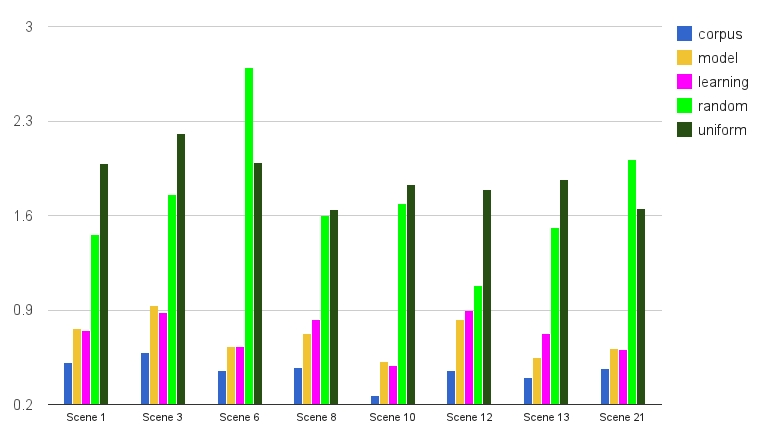
\includegraphics[width=.55\textwidth]{images/entropy.jpg}
\end{center}
\vspace*{-.5cm}
\caption{Cross-entropy between the corpus distribution and different runs of the algorithm}\label{Entropy}
\end{wrapfigure}

%Because accuracy is considered a very strict measure that in some cases can 
%be too stern on the evaluated algorithms 

We also computed the entropy of the probability distribution of REs found in the corpus, and the cross-entropy between the corpus distribution of REs and the execution of each algorithm we just described~(see~\cite{juraksky:spee08} for details on cross-entropy evaluation). Figure~\ref{Entropy} show the results for the eight scenes we are considering. 
%
%
%
The cross-entropies from the first two runs (\emph{scene} and \emph{learned}) are, in general, much closer to the corpus entropy than \emph{random}'s and \emph{uniform}'s cross-entropies, and to each other.  Only in Scene 12 \emph{random} approaches, by chance, the other two. 
%
%The figure clearly shows also that the cross entropies of \emph{scene} and \emph{learned} are in most cases very close to each other. 
%This observation supports the learning mechanism proposed in Section~\ref{sec:learning} to estimate the \puse\ when no corpora of REs of the target scene is available. 
